 \documentclass[a4paper, 12pt]{extarticle}
\usepackage[left=2.5cm, right=2.5cm,top=2.5cm,text ={18cm,25cm}]{geometry}
\usepackage[utf8]{inputenc}
\usepackage{times}
\usepackage{enumitem}
\usepackage{graphicx}
\usepackage{hhline}
\usepackage{pdflscape}
\usepackage{afterpage}
\usepackage{svg}
\usepackage{changepage}
\usepackage{amsmath}
\usepackage{adjustbox}

\newcommand\blankpage{%
    \null
    \thispagestyle{empty}%
    \addtocounter{page}{-1}%
    \newpage}

\renewcommand{\contentsname}{Obsah}
\usepackage[figurename=Graf]{caption}
\begin{document}
\begin{center} 
\thispagestyle{empty}
\Huge
\textsc{Fakulta informačních technologií\\Vysoké učení
technické v Brně}\\
\vspace{\stretch{0.167}}


\includegraphics[scale = 0.5]{fit-logo.eps}

\vspace{\stretch{0.215}}

\LARGE Technická zpráva projektu předmětu IMS\\
\Huge Varianta 4: Chov hmyzu pro potravinářské a průmyslové účely \\
\vspace{\stretch{0.218}}
\Huge
Tomáš Kukaň \\
Petr Knetl \\

\vspace{\stretch{0.400}}
\end{center}
{\LARGE \hfill
7. prosince 2018}

\newpage

\tableofcontents
\pagenumbering{arabic}
\thispagestyle{empty}
\setcounter{page}{1}
\newpage

\section{Úvod}
Tento text vznikl jako dokumentace projetku Modelování a Simulace. Zadáním bylo vytvořit a nasimulovat model$^{8}$ (slide~7.)	 hmyzí farmy v podmínkách uzemí České republiky. Naše simulace$^{8}$ (slide~7.) modeluje cvrččí farmu, konkrétně poměr cvrčků uchovaných pro vytvoření další generace ku dílu zpracovaných a prodaných jako finální produkt.

\subsection{předloha modelu a zdroje informací}
Model byl vytvořen na základě informací získaných z internetu. Veškeré zdroje jsou uvedeny na konci dokumentu v v referencích (kapitola \ref{zdroje}.). Nejdůležitějším zdrojem pro nás byl entomologický vědecký článek \textit{Methods for rearing the house cricket, Acheta domesticus (L.), along with baseline values for feeding rates, growth rates, development times, and blood composition} od dvojce autorů Craig W. Clifford a Joseph Woodring, protože se jedná o skutečný vědecký výzkum. Ostatní zdroje jsme používali s opatrností, jelikož se jedná o články z internetu ke kterým nejsou uvedeny patřičné zdroje.

\section{Rozbor tématu}
K vytvoření modelu je potřeba nejprve dobře znát a porozumět jeho předloze. Reálná cvrččí farma se zabývá chovem cvrčků pro potravinářské účely. Jedná se o velmi efektivní a udržitelný způsob produkce nutričně kvalitní potravy. V asijských zemích je tento způsob obživy naprosto normální a má svojí tradici, ale do západních zemí se teprve dostáva. Čím dál více je chov hmyzu vyzdvihován, právě kvůli udržitelnosti a celkové ekologické šetrnosti oproti chovu hospodářských zvířat. Předpokládá se, že chov hmyzu se budu čím dál více šířit, a to například z důvodu, že se hmyz letos legislativně stane povoleným jídlem v celé Evropské unii$^{5}$. V České republice se žádne velké cvrččí farmy  zatím nevyskytují, avšak v zahraničí (převážně v Thajsku) již farmy českých vlastníků existují, a cvrččí produkty se do Čech importují$^{5}$. 

\subsection{Životní cyklus cvrčků} \label{cyklus} 
Celý proces (životní cyklus generace) začíná u nakladených vajíček. Vajíčka jsou odebrána od rodičů a přesunuta do líhně, neboli do místa splňujícího podmínky na teplotu a vlhkost vzduchu. V líhni stráví vajíčka v průměru mezi deseti až čtrnácti dny. Jakmile se vajíčka vylíhnout, jsou přesunuty zpět do farmy. Další etapa ve vývojí cvrčků je dospívání. To trvá přobližně třicet dní. V průběhu dospívání je potřeba každý den cvrčkům doplňovat vodu a krmení. Voda je cvrčkům podáváná v nacucané mycí houbě, která je potřeba pro zdraví cvrčků pravidelně čistit. Jakmile cvrčci dospějí, tak většina je usmrcena zamražením a  připravena pro další zpracování, poté vcelku prodána nebo je z nich vytvořen následný produkt, převážně mouka$^{6}$. Zbytek cvrčků je nechán pro nakladení vajíček a vytvoření další generace. Pro vytvoření další generace stačí zlomek z celkových cvrčků, protože jsou při kladení vajíček velice aktivní a množí se exponenciální rychlostí. 

\newpage

\subsection{Podmínky chovu}
K produkci cvrčků je potřeba hned několik věcí. Mezi ty nejdůležitějsí patří kvalitní krmení, voda a prostory pro chov, kde lze regulovat a hlavně udržovat správnou teplotu a vlhkost vzduchu. Pro správný růst a zdraví cvrčků je potřeba zachovávat teplotu v místnosti mezi dvacetisedmy až třicetidvěma stupni Celsia a vlhkost vzduchu mezi třiceti až padesáti procenty. Pro líhnutí vajíček jsou podmínky ještě přísnější. Na kvalitní vylíhnutí je potřeba udržovat vlhkost blízko sto procentům a teplota nesmí klesnout pod dvacetsedm stupňů Celsia$^{6}$.


\section{Konceptuální návrh}
Náš návrh konceptuálního modelu$^{8}$ (slide 48.) se soustředí na  poměr zpracovaných cvrčků, a těch kteří jsou ušetřeni pro vytvoření další generace. V závislosti na této proměnné sledujeme finanční výnos chovu. Pro takovouto simulaci není potřeba kompletní model farmy, tudíž jsou něteré části zanedbány a model je zjednodušen. Například v našem modelu nedochází ke krmení cvrčků každý den, nýbrž je finanční suma stržena až po celém životním cyklu cvrčků. Návrh modelu je v podobě Petriho sítě zobrazen na obrázku \ref{petrinet}. Zobrazená Petriho síť modeluje případ, kdy prodáváme 90\% cvrčků a 10\% uchováváme pro reprodukci.\\

\begin{figure}[h]
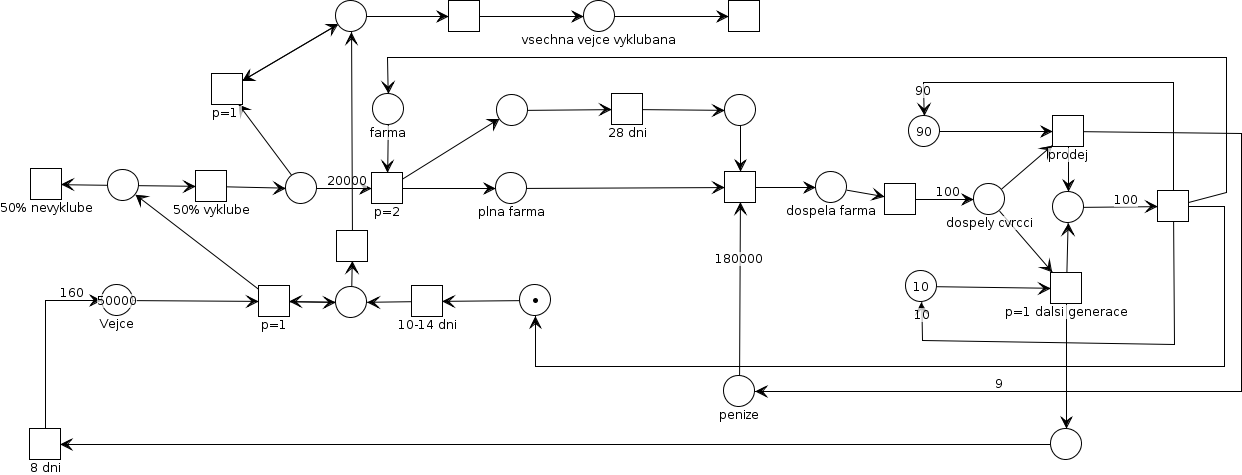
\includegraphics[width=\linewidth]{IMS2.png}
\caption{Zobrazení modelu pomocí Petriho sítě} \label{petrinet}
\end{figure}

Model je činný po dobu jednoho roku simulovaného času. Počítáme s tím, že farma nemůže být nekonečně velká, proto jsme zvolili 20 000 cvrčků jako maximální limit farmy. Poté co cvrčci vyrostou, tak je necháváme klást vajíčka dalších 8 dní a poté startujeme další cyklus (generaci).

\newpage

\subsection{Poměr prodaných ku poměru reprodukčních} 
Jak již bylo řečeno v kapitole \ref{cyklus}, tak cvrčci se množí exponenciální rychlostí díky obrovské frekvenci kladení vajíček. To umožňuje po dospění velkou část generace usmrtit a prodat, zatímco si jen zlomek dospělých cvrčků necháme pro početí další generace.V našem výzkumu zkoumáme právě ideální poměr pro maximalizování výnosu farmy. 

Čím více cvrčků se okamžitě po dospění prodá, tím větší okamžitý zisk vznikne, avšak z dlouhodobého hlediska to může být prodělečné, z důvodu nedostatku snesených vajíček a vytvoření příliš malé další generace. Nadruhou stranu pokud necháme příliš moc cvrčků pro tvoření další generace, tak okamžitý zisk snížíme a navíc musíme uvažovat s útratou na krmení ponechaných cvrčků. Další důležitou proměnnou modelu je fakt, že kapacita cvrččí farmy není nekonečná, tudíž vylíhnuté cvrčky, kteří se už do farmy nevejdou, nelze chovat a o potenciální zisk tak přijdeme.

\subsection{Číselné hodnoty modelu}
V našem modelu bylo použito hned několik konstant, které vycházejí z referenčních zdrojů. Tyto konstanty jsou: 
\begin{enumerate}
\item Nákupní cena 100 vajec$^{4}$	-	14.3,- Kč
\item Prodejní cena 100 cvrčků$^{3}$	-	195.8,- Kč
\item Úspěšnost vylíhnutí vejce$^{4}$	-	50\%
\item Doba inkubace vejce$^{1}$ 	-	10 až 14 dní
\item Doba dospívání cvrčka$^{3}$ -  	28 dní
\item Počet nakladených vajec crvček/den$^{1}$ - 20 vajec
\end{enumerate}

\section{Implementace}
Simulace byla vytvořena v programovacím jazyku \texttt{C++} s využitím knihovny \texttt{SIMLIB}$^{9}$. Jazyk byl zvolen z důvodu využití objektového návrhu aplikace. Části programu jsou převzaty z přednášek a demostračních příkladů předmětu IMS. Jedno spuštění programu vygeneruje data pro konrétní nastavení poměru prodaných:zachovaných cvrčků. Pro opakované spustění jsem napsali Python script \texttt{get\_statistics.py}, který spouští simulaci s ruznými vstupy a výstupy ukládá do csv souboru. Z csv souboru jsou následně vygenerováný grafy z kapitoly \ref{zaver}.

\subsection{Simulační model}
Model byl simulován pomocí několika instancí třídy \texttt{Proccess}$^{9}$ knihovny \texttt{Simlib}. Proces byl vytvořen pro farmu, generátor vajec, vejce, mláďata a rodiče (dospělé cvrčky). Implementace odpovídá nákresu \ref{petrinet}. Simulace začíná zakoupením (vygenrováním) vajec, které jsou následně přesunuty do instance Líheň třídy \texttt{Store}$^{9}$. Jakmile jsou všechna vejce vyklubána, jsou přesunuta do farmy. Proces farmy simuluje čas dospívání cvrčků a cenu za jejich krmení. Poté co cvrčči dospějí, je část okamžitě prodána a zbytek je přesunut do procesu Rodič. Proces simuluje kladení vajíček v průběhu času. Po ukončení procesu Rodič se řízení programu přesouvá zpět do procesu Vejce a tak simulace pořád dokola iteruje až do dosažení času jednoho roku, kdy končí.

\newpage

\section{Experiment}
Experiment spočíval v opakovaném spouštění modelu s jinými hodnotami vstupní proměnné (poměr prodaných:zachovaných cvrčků). Proměnnou jsme měnili v intervalu mezi nulou až sto procenty. v itervalu nula až devadesát jsme stanovili krok pět procent, protože zhuštění vzorku na tomto intevalu by nepřineslo žádné další užitečná data. Vzorkovaní jsme avšak změnili v intevalu devadesát až sto procent na délku kroku jedno procento. Z toho intervalu je totiž možno vyvodit závěr kolik procent cvrčků je výhodné si ponechat a kolik jich prodat. 


\section{Shrnutí výsledků} \label{zaver}

\subsection{Inerval od 0 do 90{\%}}
Výsledky z tohoto intervalu jsou zobrazeny v grafu \ref{chart1}. Osa x zobrazuje zisk/ztrátu peněz v Českých korunách, osa y zobrazuje procento prodaných cvrčků. Z grafu je zjevné, že pokud prodáme pouze šest procent nebo méně cvrčků, pak zůstane přilíš moc cvrčků pro vytvoření další generace a vznikne přebytečné množství vajec, které nebude možné využít kvůli omezené kapacitě farmy. Jakmile prdáme více než šest procent cvřků, pak začne být farma výdělečné, avšak velice málo oproti jejímu plnému potenciálu. Od šesti do devadesáti procent se funkce nemění a roste lineárně. Čím více vajec na tomto intervalu prodáme, tám větší zisk vznikne. Funkce se začne zajímavě chovat v okolí 98\%, viz. další podkapitola.


\begin{figure}[h]
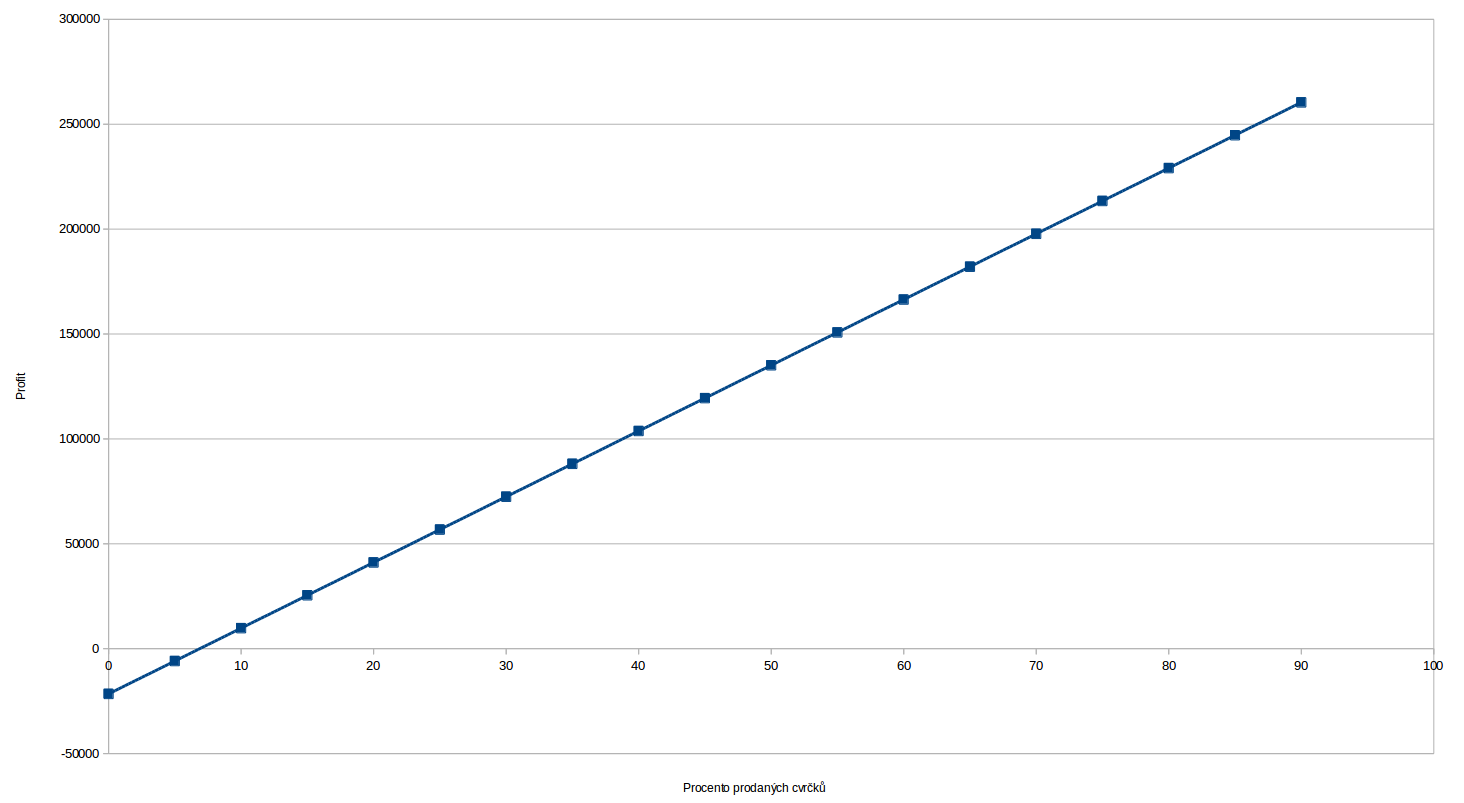
\includegraphics[width=\linewidth]{chart1.png}
\caption{Interval mezi 0 a 90\% prodaných cvrčků} \label{chart1}
\end{figure}

\newpage
\subsection{Inerval od 90 do 100{\%}}
Průběh tohoto intervalu zobrazuje graf \ref{chart2}. Osa x opět zobrazuje zisk/ztrátu peněz v Českých korunách a osa y zase zobrazuje procento prodaných cvrčků. Funkce stále strmě lineárně stoupá až k 98\% prodaných cvrčků, kde je výnos maximální. Jakmile ovšem překročíme tuto hranici, zisk kolmě klesat. Funkce takto klesá z důvodu nedostatku vzniklých vajíček pro další generaci. Chybějící vajíčka jsme nuceni dokoupit a na tom farma tratí.

\begin{figure}[h]
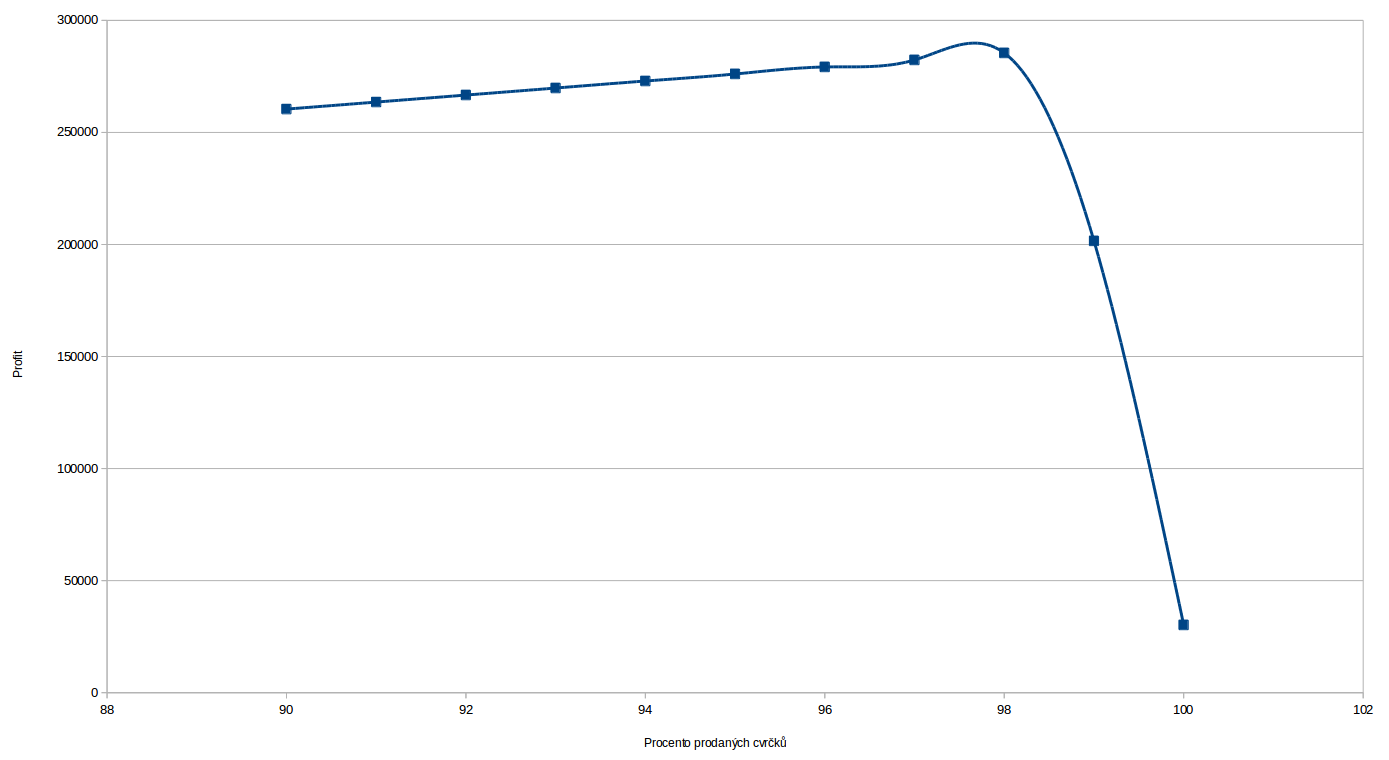
\includegraphics[width=\linewidth]{chart2.png}
\caption{Interval mezi 90 a 100\% prodaných cvrčků} \label{chart2}
\end{figure}

\newpage
\subsection{Vliv procenta prodaných cvrčků na ztrátu vajec a cvrčků}
 Tento vztah zobrazuje graf \ref{chart3}. Osa Y zobrazuje pro jednotlivé funkce zisk/ztrátu peněz (tentokrát v amerických dolarech pro lepší přehlednost), počet nevyužitých vajec a počet nevyužitých mláďat. Osa x osa  opět zobrazuje procento prodaných cvrčků v intervalu devadesát až sto procent. Z grafu je opět vidět že k maximálnímu zisku dojde pří prodání 98\% procent cvrčků a to z důvodu stoprocentního využití vajec. Vajec je v tomto nastavení vhodný počet, protože po vylíhnutí existuje dosatek cvčků pro naplnění farmy, ale zároveň se téměř všichni cvrčci vejdou do farmy a nedochází k jejich plýtvání.

\begin{figure}[h]
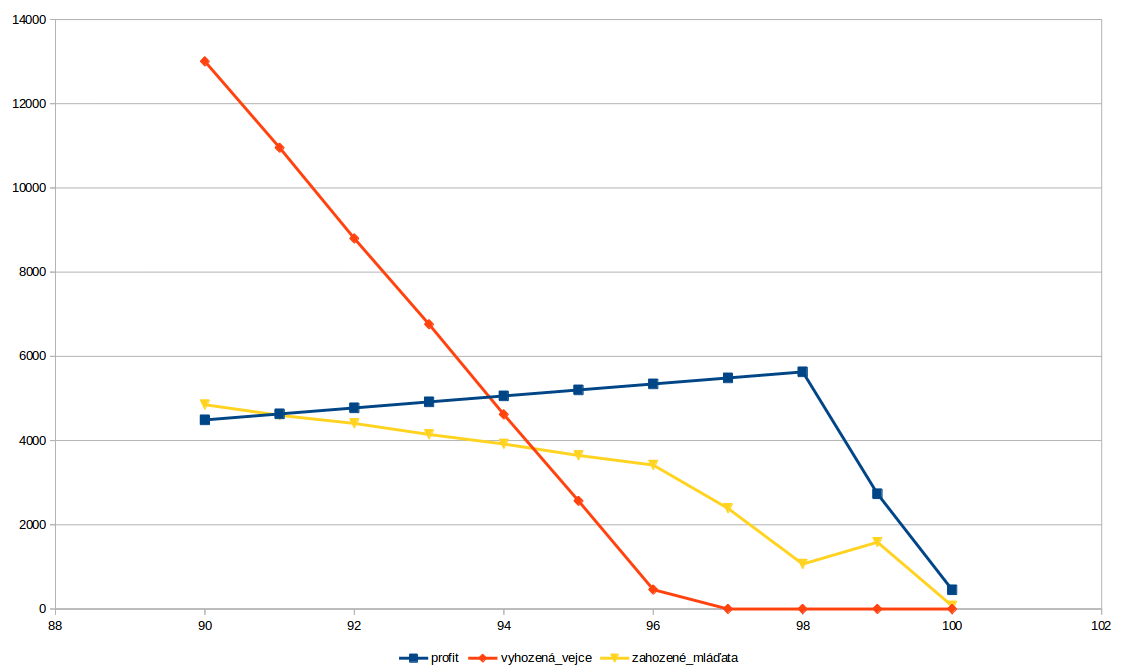
\includegraphics[width=\linewidth]{chart3.png}
\caption{Interval mezi 90 a 100\% prodaných cvrčků} \label{chart3}
\end{figure}

\section{Závěr}
Zkoumáním simulačního modelu bylo zjištěno že ideálním poměrem prodaných a zachovaných cvrčků je devadesátosm ku dvoum procentům pro výše uvedené hodnoty. Pokud by se parametry farmy lišili, musel by se experiment provést znovu.

\newpage

\section{Zdroje informací} \label{zdroje}
\setlength\parindent{0pt}

[1] WOODRING J.P., Clifford C.W. Methods for rearing the house cricket, Acheta domesticus (L.), along with baseline values for feeding rates, growth rates, development times, and blood composition. USA, 1990.\\

[2] Feeder Crickets. A Quick Run Down of a Cricket's Life Cycle. The Critter Depot. [online]. 2018, [cit. 2018-12-06]. Dostupné z: https://www.thecritterdepot.com/blogs/news/34185665-a-quick-run-down-of-a-crickets-life-cycl\\

[3] Fluker's Cricket Farm. Live Crickets Farm - Order Online. Fluker's Cricket Farm. [online]. 2018, [cit. 2018-12-06]. Dostupné z: https://flukerfarms.com/live-crickets/ \\

[4] Premium Crickets. Bulk Cricket Eggs. The Premium crickets. [online]. 2018, [cit. 2018-12-06]. Dostupné z: http://www.premiumcrickets.com/Products/Bulk-Cricket-Eggs-approximately-60-000\_\_eggs.aspx \\

[5] PATOČKOVÁ, Martina. Stamiliony cvrčků pro Evropu. Češi otevřou největší hmyzí farmu na světě. Idnes [online]. 2018, [cit. 2018-12-06]. Dostupné z: https://ekonomika.idnes.cz/hmyz-jidlo-potravina-crvcci-d1j-/ekonomika.aspx?c=A180204\_094800\_ekonomika\_ane\\

[6] KOIVU TELEVISION. KoivuTV and Johanna Koivu gets acquainted with a Finnish cricket farm [Video File]. 2018, [cit. 2018-12-06]. Dostupné z https://youtu.be/gNG7lOFBM8\\

[7] COWBOY CRICKETS. Cricket Farming For Food and Feed [Video File]. 2018, [cit. 2018-12-06]. Dostupné z https://youtu.be/JUgDsxWYSS8\\

[8] PERINGER, Petr. Modelování a simulace [online]. 2017, [cit. 2018-12-06]. Dostupné z:\\ https://wis.fit.vutbr.cz/FIT/st/cfs.php?file=\%2Fcourse\%2FIMS-IT\%2Flectures\%2FIMS.pdf\\\&cid=12760 \\

[9] PERINGER, Petr. Popis simulační knihovny SIMLIB [online]. 1997, [cit. 2018-12-06]. Dostupné z: https://www.fit.vutbr.cz/~peringer/SIMLIB/doc/html-cz/





\end{document}